\begin{center}
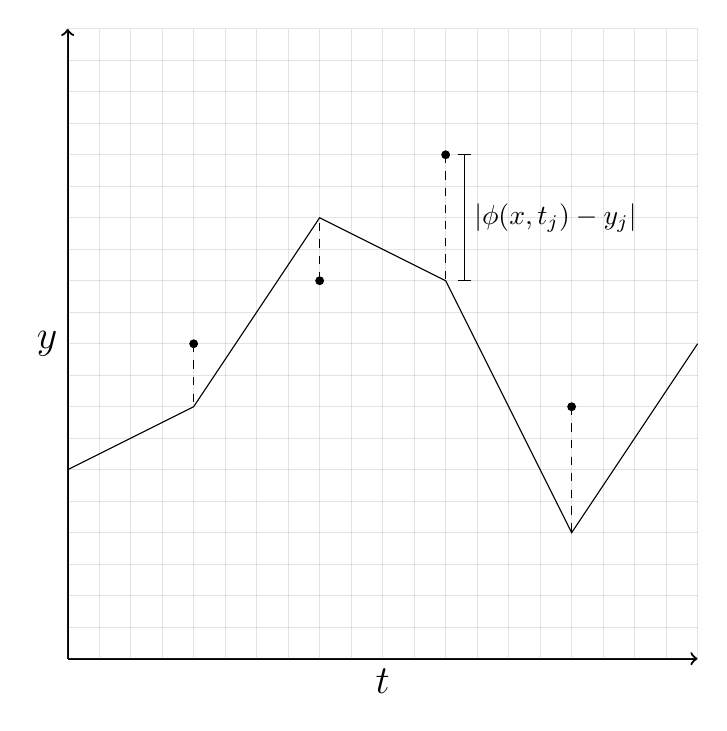
\begin{tikzpicture}
	[scale=0.8,
	axis/.style={->,black,thick}]
	
	
	% Draw main axes
	\draw[axis] (0,0) -- (10, 0) node[midway, below] {\Large $t$};
	\draw[axis] (0,0) -- (0, 10) node[midway, anchor=east] {\Large $y$};
	
	%\clip (0,0) rectangle (10, 10);
	
	% Draw grid
	\foreach \x in {0,0.5,...,10}
		\foreach \y in {0,0.5,...,10}
		{
			\draw[thin, gray, opacity=0.01] (\x, 0) -- (\x, 10);
			\draw[thin, gray, opacity=0.01] (0, \y) -- (10, \y);
		}
	
	% Draw model
	\draw[] (0,3) -- (2, 4) -- (4,7) -- (6,6) -- (8,2) -- (10, 5);
	
	% Draw measurements
	\fill (2, 5) circle[radius=2pt];
	\draw[dashed] (2,5) -- (2,4);
	
	\fill (4, 6) circle[radius=2pt];
	\draw[dashed] (4,6) -- (4,7);

	\fill (6, 8) circle[radius=2pt];
	\draw[dashed] (6,8) -- (6,6);
	\draw[] (6.2, 8) -- (6.4,8);
	\draw[] (6.2, 6) -- (6.4,6);
	\draw[] (6.3, 6) -- (6.3,8) node[midway, anchor=west] {$|\phi(x,t_j)-y_j|$};
	%\draw[decoration={brace, raise=0pt}, decorate]
		(6,8) -- (6,6) node[midway, anchor=west] {\scriptsize Interval 1};
	
	\fill (8, 4) circle[radius=2pt];
	\draw[dashed] (8,4) -- (8,2);
	
	
	
	
	
	
	
	
	
	
	
	
\end{tikzpicture}
\end{center}